\documentclass[10pt,twocolumn,letterpaper]{article}

\usepackage{cvpr}
\usepackage{times}
\usepackage{epsfig}
\usepackage{graphicx}
\usepackage{amsmath}
\usepackage{amssymb}
\usepackage{subfig}
% Include other packages here, before hyperref.

% If you comment hyperref and then uncomment it, you should delete
% egpaper.aux before re-running latex.  (Or just hit 'q' on the first latex
% run, let it finish, and you should be clear).
%\usepackage[pagebackref=true,breaklinks=true,letterpaper=true,colorlinks,bookmarks=false]{hyperref}

\cvprfinalcopy % *** Uncomment this line for the final submission

\def\cvprPaperID{****} % *** Enter the CVPR Paper ID here
\def\httilde{\mbox{\tt\raisebox{-.5ex}{\symbol{126}}}}

% Pages are numbered in submission mode, and unnumbered in camera-ready
%\ifcvprfinal\pagestyle{empty}\fi
\setcounter{page}{4321}
\begin{document}

%%%%%%%%% TITLE
\title{Using GelSight Sensor for Material Recognition in the Wild}

\author{Tejas D Kulkarni\\
Massachusetts Institute of Technology\\
{\tt\small tejask@mit.edu}
}

\maketitle
%\thispagestyle{empty}

%%%%%%%%% ABSTRACT
\begin{abstract}
Humans can rapidly categorize materials such as fabric, wood, metal and plastic by using visual or tactile sensory systems. Material perception
has been widely studied as a visual recognition problem. As per our knowledge, most of the work in material 
perception uses visual data -- often neglecting other sensory data such as tactile feedback. This neglect is 
primarily due to lack of easy availability of tactile sensors. GelSight is a novel tactile sensor technology that can
provide detailed and rapid surface measurements of any physical object. We use GelSight sensor to create a dataset of
material categories from real world objects that include -- Fabrics, Foliage, Stones and Wood. We primarily collect RGB
images depicting the microscopic view of materials and also the 3D reconstruction of the surface properties of the material
through the GelSight sensor. We propose using globally weighted Linear Binary Pattern $(LBPV)$ features and 3D shape features $(SF)$ to classify
material category for novel data. The classification rate using our proposed algorithms is: Fabrics, Foliage, Stones and Wood. 
It is clearly evident from the LBPV classification results that material perception through tactile data
is not just a texture problem but needs 3D shape information for some material categories. 
\end{abstract}


%%%%%%%%% BODY TEXT
\section{Introduction}
One of the goals of the human visual system is to infer rich structural properties of the world from visual scenes. In order to infer these properties, 
the visual cortex can semantically and syntactically parse visual scenes. Object recognition is one way to realize such a scene parser -- where the visual cortex
could aggregate detected objects to form perception. On the other hand, there is a lot of visual $stuff$ in the world which cannot be handled by current object 
recognition systems. For example, a leather and plastic shoe belong to the same object cateogry but not the same material category. 

\begin{figure}[h]
\minipage [c]{0.15\linewidth}

\includegraphics[width=\linewidth]{images/fabric.png}
\endminipage\hfill
\minipage [c]{0.15\linewidth}
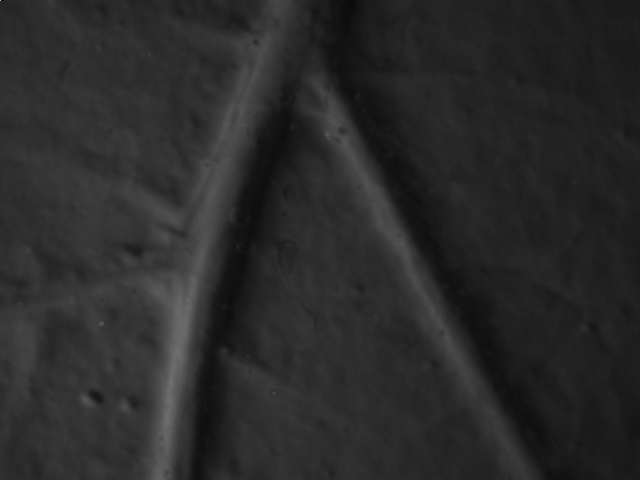
\includegraphics[width=\linewidth]{images/foliage.png}
\endminipage\hfill
\minipage [c]{0.15\linewidth}

\includegraphics[width=\linewidth]{images/stone.png}
\endminipage\hfill
\minipage [c]{0.15\linewidth}
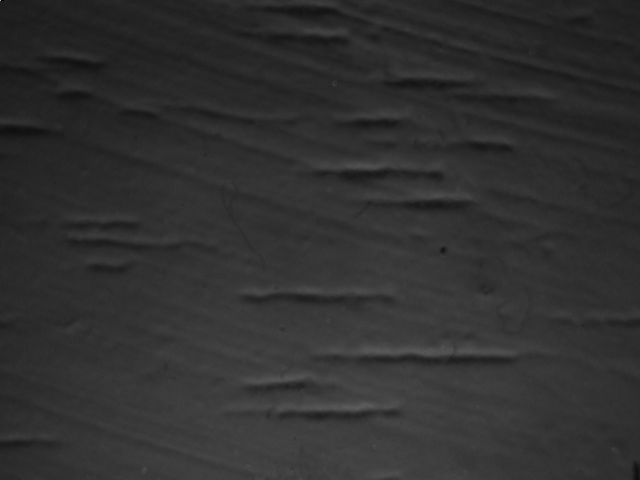
\includegraphics[width=\linewidth]{images/wood.png}
\endminipage\\

\minipage [c]{0.25\linewidth}
\includegraphics[width=\linewidth]{images/fabric.eps}
\endminipage\hfill
\minipage [c]{0.25\linewidth}
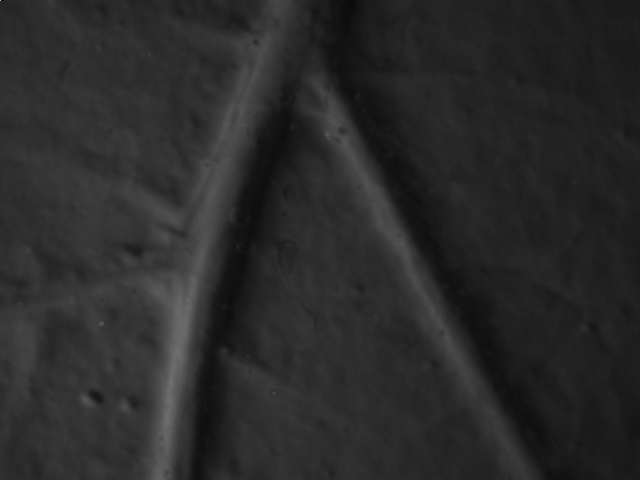
\includegraphics[width=\linewidth]{images/foliage.eps}
\endminipage\hfill
\minipage [c]{0.25\linewidth}
\includegraphics[width=\linewidth]{images/stone.eps}
\endminipage\hfill
\minipage [c]{0.25\linewidth}
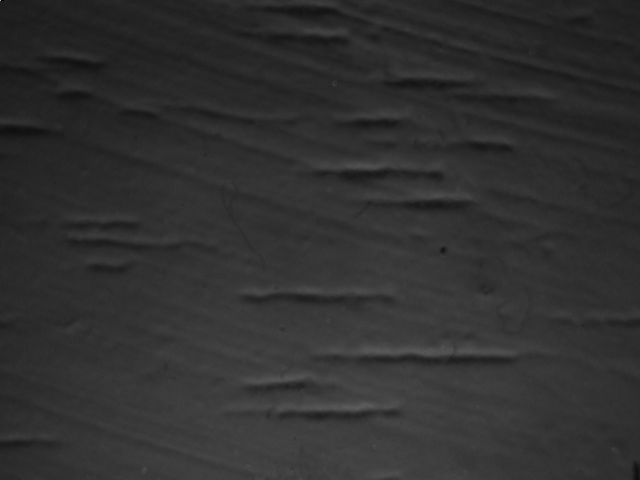
\includegraphics[width=\linewidth]{images/wood.eps}
\endminipage\\

\caption{TODO}
\end{figure}


\begin{figure*}[t]
\centering
	\includegraphics[width=0.8\linewidth]{images/gelnew.eps}
   \caption{TODO }
\end{figure*}


Humans can infer material categories by $looking$ and $touching$ physical objects. However, material recognition using tactile data has been largely unexplored. 
However, with the advent of GelSight sensor, which can provide cheap, fast and robust surface measurements from objects, it has now become possible to tackle this 
problem in the tactile domain (Fig 1). The GelSight sensor has a proprietary gel that deforms in accordance with the physical object that it touches at any given
point of time. This gel magnifies the surface of the object and "covers" it with it's own surface BRDF. A camera overlooking this gel takes six photographs,
where in each photograph, the light direction that illuminates the gel varies it's source direction automatically. A photometric stereo method developed by [?] can then
by used to obtain the 3D reconstruction of the surface properties of the object. 

We use both the RGB and 3D shape images obtained from the GelSight sensor and propose two different material classification algorithms. The RGB images (Fig 2) obtained
from the sensor are under varying illumination conditions. We fix the illumination condition and construct a dataset of such images for different material categories.
These images reflect the microscopic structure of materials under known BRDF, which is calculated by a calibration technique given in [?]. Given this image dataset,
the problem of material classification can be posed as a texture recognition problem. We use LBPV features, proposed by [?], to encode texture. Linear Binary Pattern 
(LBP) features are widely used to encode local texture properties. Authors of [?] have recently proposed weighted LBP, which is called as LBPV, which uses global variances
as weights for LBP value at each pixel. Thus LBPV capture the local as well as global texture properties in an image. We use a supervised learning algorithm (SVM) to
learn a material classifier using LBPV features. We learnt that for material categories without repeating patterns (Fig 3), textures do not provide a 
good feature representation to perform material classification. This led us to use 3D shape information to classify material categories. The main contributions of 
this paper are: 
\begin{itemize}
\item One of the first attempts to model tactile based material perception as a vision problem for challenging material categories
\item Best features to encode GelSight data for material recognition
\item Real-time execution of material classification, which is important for robotics applications among others. 
\item Challenges current view that tactile based material perception is primarily a texture problem. Results indicate that additional information
such as 3D shape may be very important.
\end{itemize}

%-------------------------------------------------------------------------
\section{Related Work}
Several groups have been trying to solve material recognition using visual data [?]. One of the leading methods to classify materials make use of bayesian inference
to detect materials from images [?]. In this method, several discriminative features such as SIFT and color are used, and the clusters of these features are modelled using LDA for classification.
On the other hand, we are not aware of direct work done in material perception using tactile information alone. This is primarily due to the lack of availability of good sensors to capture tactile data. 
With GelSight, it has been very easy and cheap to get access to such tactile data and model it as a vision problem. Additionally, various groups have studied texture recognition, which is interesting
for tactile based material perception ~\cite{textons,lbpv}. We shall use ideas from ~\cite{lbpv} to build one of the features for our material classifier. 







%-------------------------------------------------------------------------





\subsection{Miscellaneous}

\noindent
Compare the following:\\
\begin{tabular}{ll}
 \verb'$conf_a$' &  $conf_a$ \\
 \verb'$\mathit{conf}_a$' & $\mathit{conf}_a$
\end{tabular}\\



%------------------------------------------------------------------------
\section{Our Approach}
Material recognition is an important human perception problem. As described earlier, there are several methods to build a material classifier using visual data. However, humans are also able to infer
material categories by the sensation of $touch$. We shall explore the limitations of tactile based material perception using a simple test that we will refer to as the \textbf{black-box text}. 
We performed a crude psychophysics experiment with a few human subjects to test the limits of tactile based material perception. From the perspective of tactile perception, the following surface properties are
very important ~\cite{lisathesis}: 
\begin{itemize}
\item The surface profile of the material indicated by roughness/smoothness. Hereforth, all our experiments and computational algorithms will assume that these properties can vary.
\item The surface temperature/conductance of material. We will assume that these quantities are static. 
\end{itemize}

Thus under the given assumptions, we are interested in figuring out the classification rate of human subjects in discriminating between material categories purely by tactile perception. In our experiment, we placed four
different boxes with four material categories (foliage, fabrics, wood and stone). The subjects were only allowed to touch the materials, while the materials were not visible due to the compactness of the box. We observed that
the human subjects were able to perfectly categorize materials under the assumed conditions. This motivated us to wonder whether it is possible to build a material classifier using tactile data alone. Given GelSight provides 
tactile data under our assumed conditions, it allows us to tackle this question in a systematic way. 

\subsection {Dataset} 
We generated a relatively big dataset compromising of five material categories - fabrics, foliage, wood, stone and random. The $random$ category was mainly to test the false positive rate.
We collected about 150 sets of images, where each set compormised of 6 different images under varying illumination direction. Thus the total number of training/testing images were 900. The training and testing image set
were in the range of 15-25 sets (90 images to 150 images) each. We used an ensemble of exemplar SVMs to seprately train each material category. Please refer to ~\cite{exemplar} for details on the SVM training technique. 
For each set (6 images), we calculated the 3D reconstructed image using photometric stereo methods given in ~\cite{micah}.

\subsection {Calibration} 



\begin{figure}[ht]
\minipage [c]{0.33\linewidth}

\includegraphics[width=\textwidth]{images/coin1.png}
\endminipage\hfill
\minipage [c]{0.33\linewidth}

\includegraphics[width=\textwidth]{images/coin2.png}
\endminipage\hfill
\minipage [c]{0.33\linewidth}
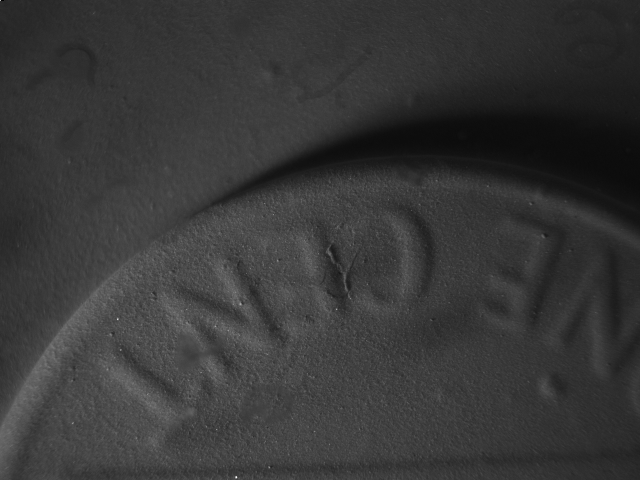
\includegraphics[width=\textwidth]{images/coin3.png}
\endminipage\\

\minipage [c]{0.33\linewidth}
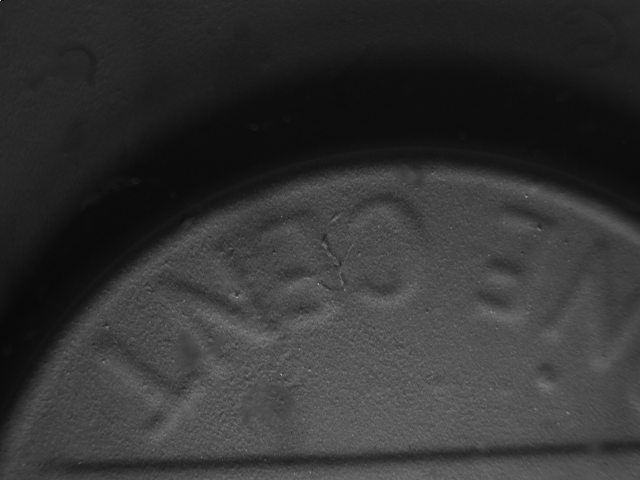
\includegraphics[width=\textwidth]{images/coin4.png}
\endminipage\hfill
\minipage [c]{0.33\linewidth}
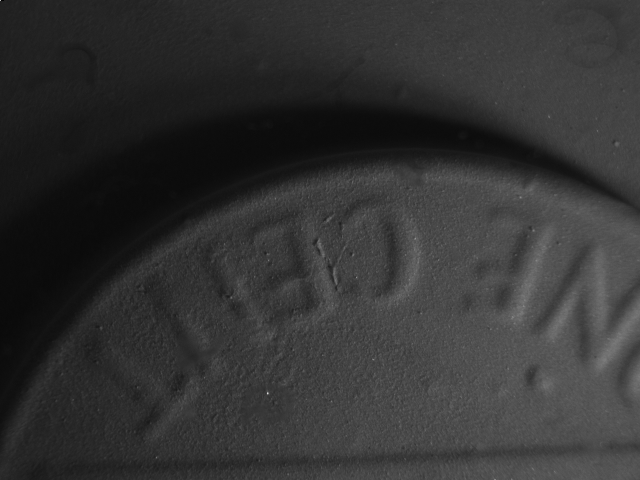
\includegraphics[width=\textwidth]{images/coin5.png}
\endminipage\hfill
\minipage [c]{0.33\linewidth}

\includegraphics[width=\textwidth]{images/coin6.png}
\endminipage\\

\caption{TODO}
\end{figure}








\begin{figure}[ht]
\minipage [c]{0.33\linewidth}
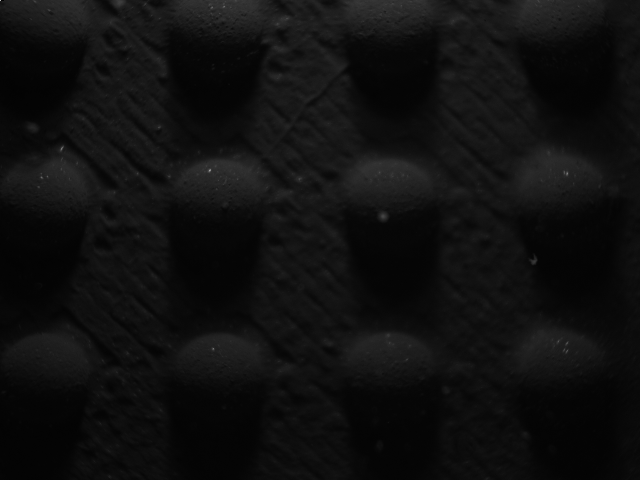
\includegraphics[width=\textwidth]{images/circle.png}
\endminipage\hfill
\minipage [c]{0.33\linewidth}
\includegraphics[width=\textwidth]{images/calib1.eps}
\endminipage\hfill
\minipage [c]{0.33\linewidth}
\includegraphics[width=\textwidth]{images/calib2.eps}
\endminipage\\

\caption{TODO}
\end{figure}


\subsection {3D Shape Features}
TODO

\begin{figure}[ht]
\minipage [c]{0.33\linewidth}

\includegraphics[width=\textwidth]{images/fabric_mask_image.png}
\endminipage\hfill
\minipage [c]{0.33\linewidth}
\includegraphics[width=\textwidth]{images/fabric_mask_shape.eps}
\endminipage\hfill
\minipage [c]{0.33\linewidth}
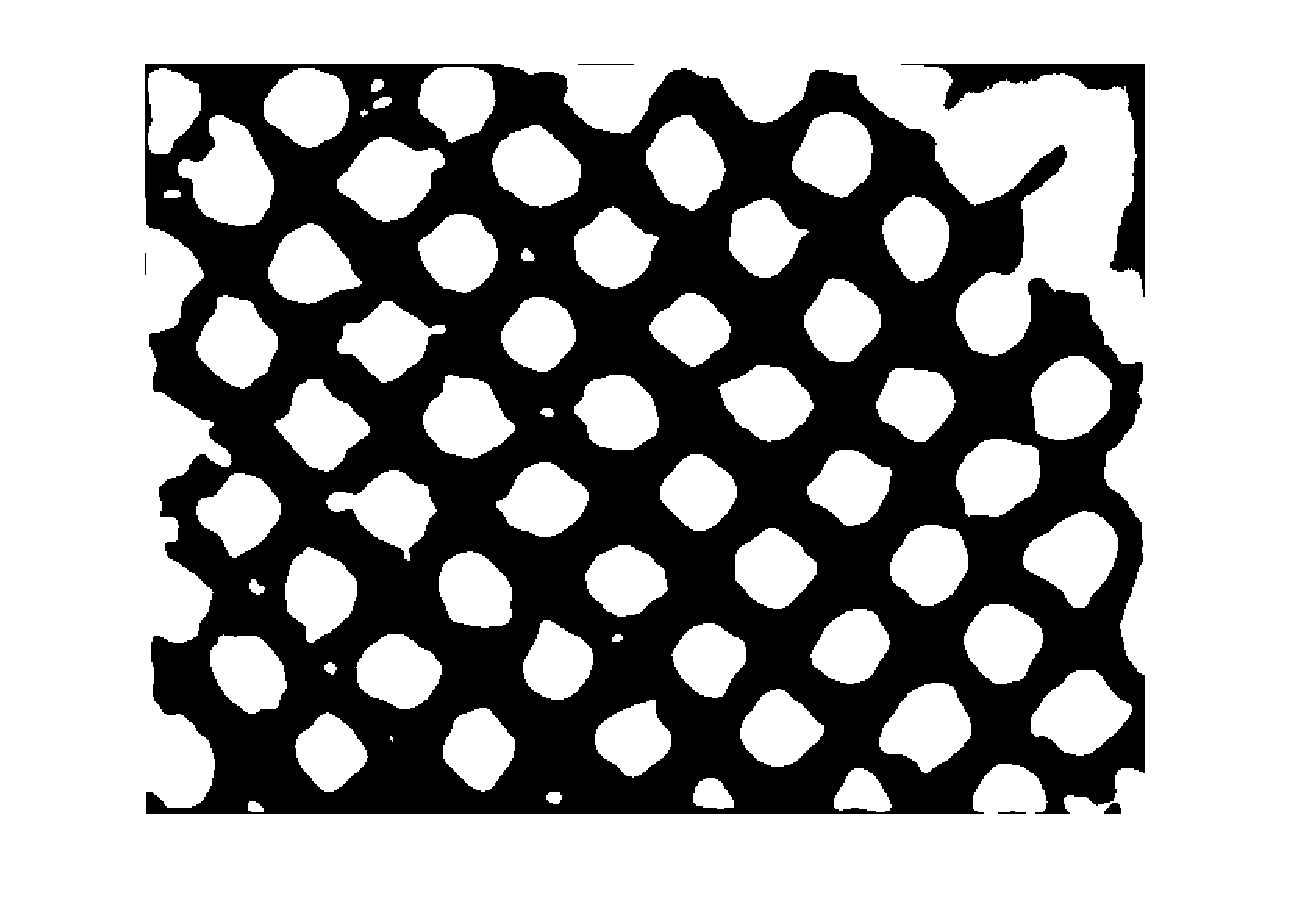
\includegraphics[width=\textwidth]{images/fabric_mask.eps}
\endminipage\\

\caption{TODO}
\end{figure}




\subsection{Classification Performance}
TODO

\begin{figure}[t]
\begin{center}
   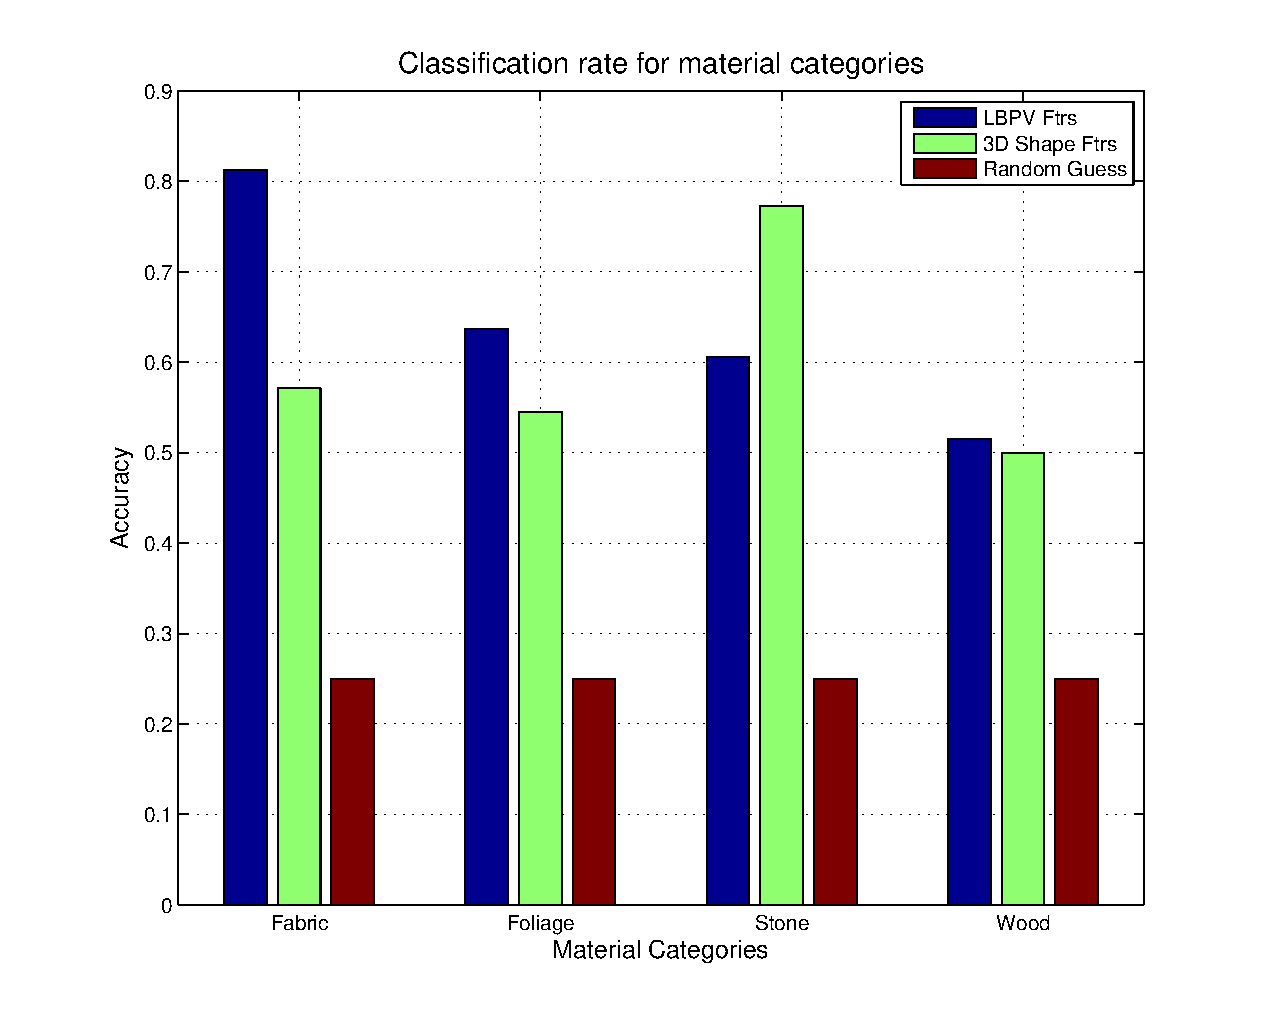
\includegraphics[width=0.8\linewidth]{images/performanceFigure.eps}
\end{center}
   \caption{TODO}
\label{fig:long}
\label{fig:onecol}
\end{figure}


\begin{figure}[t]
\begin{center}
   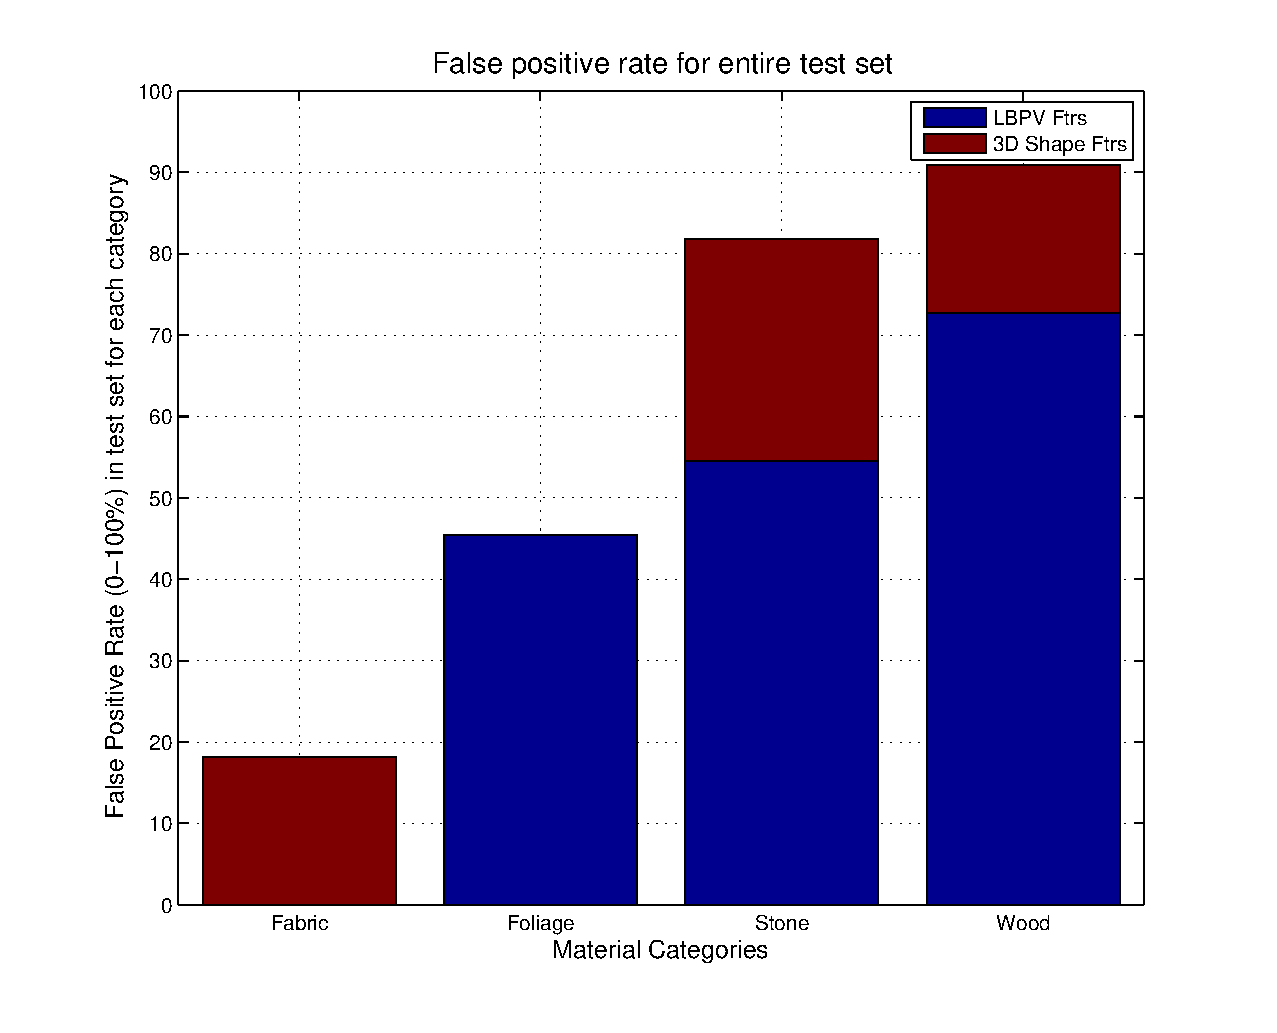
\includegraphics[width=0.8\linewidth]{images/falsepos.eps}
\end{center}
   \caption{TODO}
\label{fig:long}
\label{fig:onecol}
\end{figure}

\subsection Fast LBP Implementation
TODO

\begin{figure}[t]
\begin{center}
   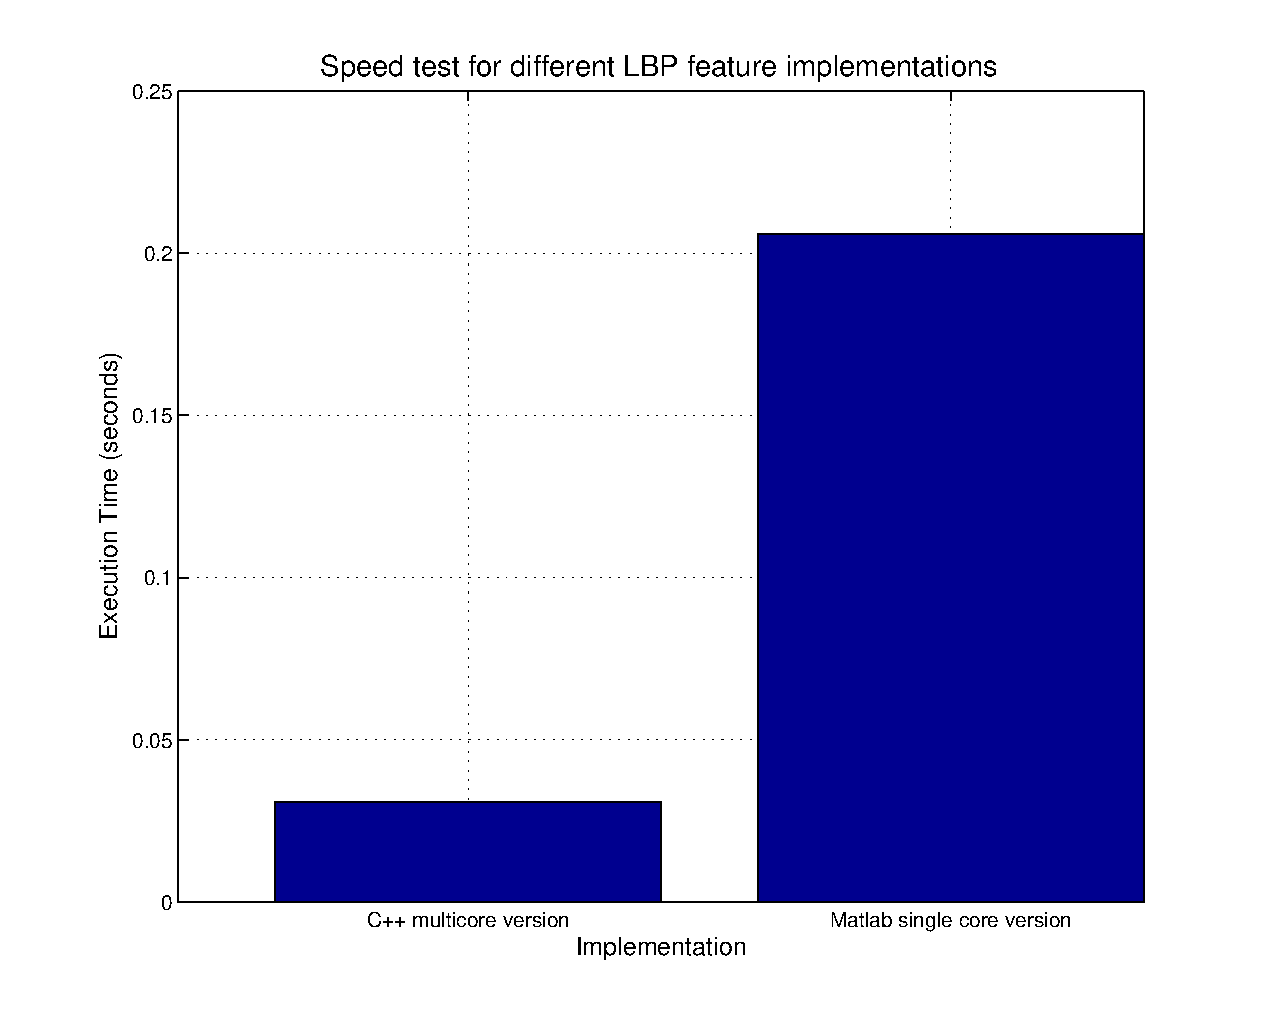
\includegraphics[width=0.8\linewidth]{images/speed.eps}
\end{center}
   \caption{TODO}
\label{fig:long}
\label{fig:onecol}
\end{figure}
%------------------------------------------------------------------------
\section{Experimental Results}
TODO

\subsection Failures

\begin{figure*}[t]
\minipage[c]{0.24\textwidth}
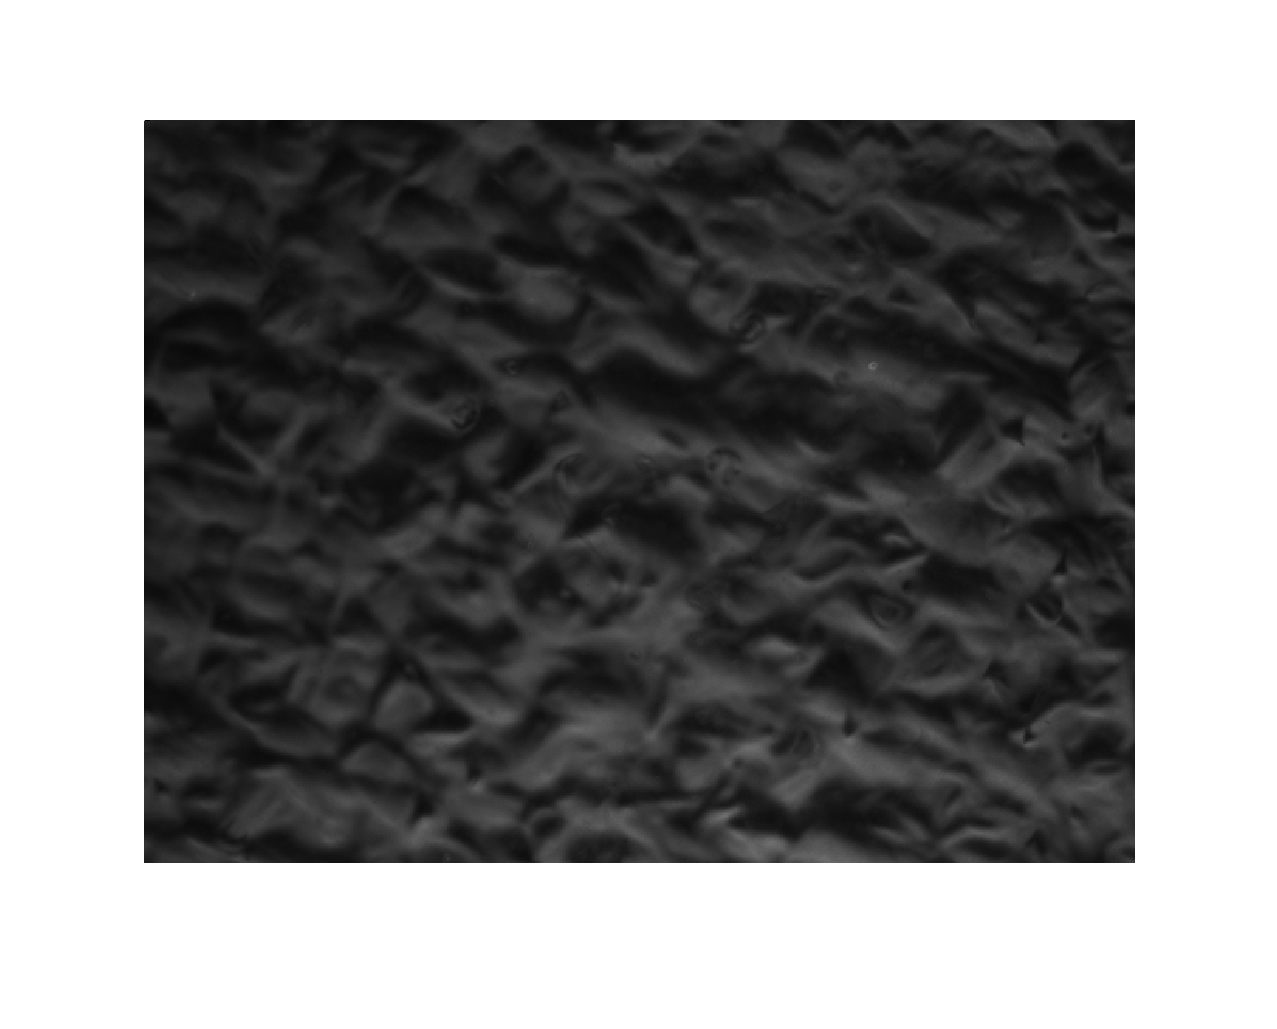
\includegraphics[width=\textwidth]{images/fail_fabric_lbp.eps}
{\small (a) MH with blur and displaying "left" RV of one box}
\endminipage\hfill
\minipage[c]{0.24\textwidth}

\includegraphics[width=\textwidth]{images/fail_fabric2_lbp.eps}
{\small (b) Gibbs with blur and displaying "left" RV of one box}
\endminipage\hfill
\minipage[c]{0.24\textwidth}
\includegraphics[width=\textwidth]{images/fail_fabric1_shape.eps}
{\small (c) MH without blur and displaying "left" RV of one box}
\endminipage\hfill
\minipage[c]{0.24\textwidth}
\includegraphics[width=\textwidth]{images/fail_fabric2_shape.eps}
{\small (d) MH sampling without blur and displaying "left" RV of one box}
\endminipage\\

\minipage[c]{0.24\textwidth}
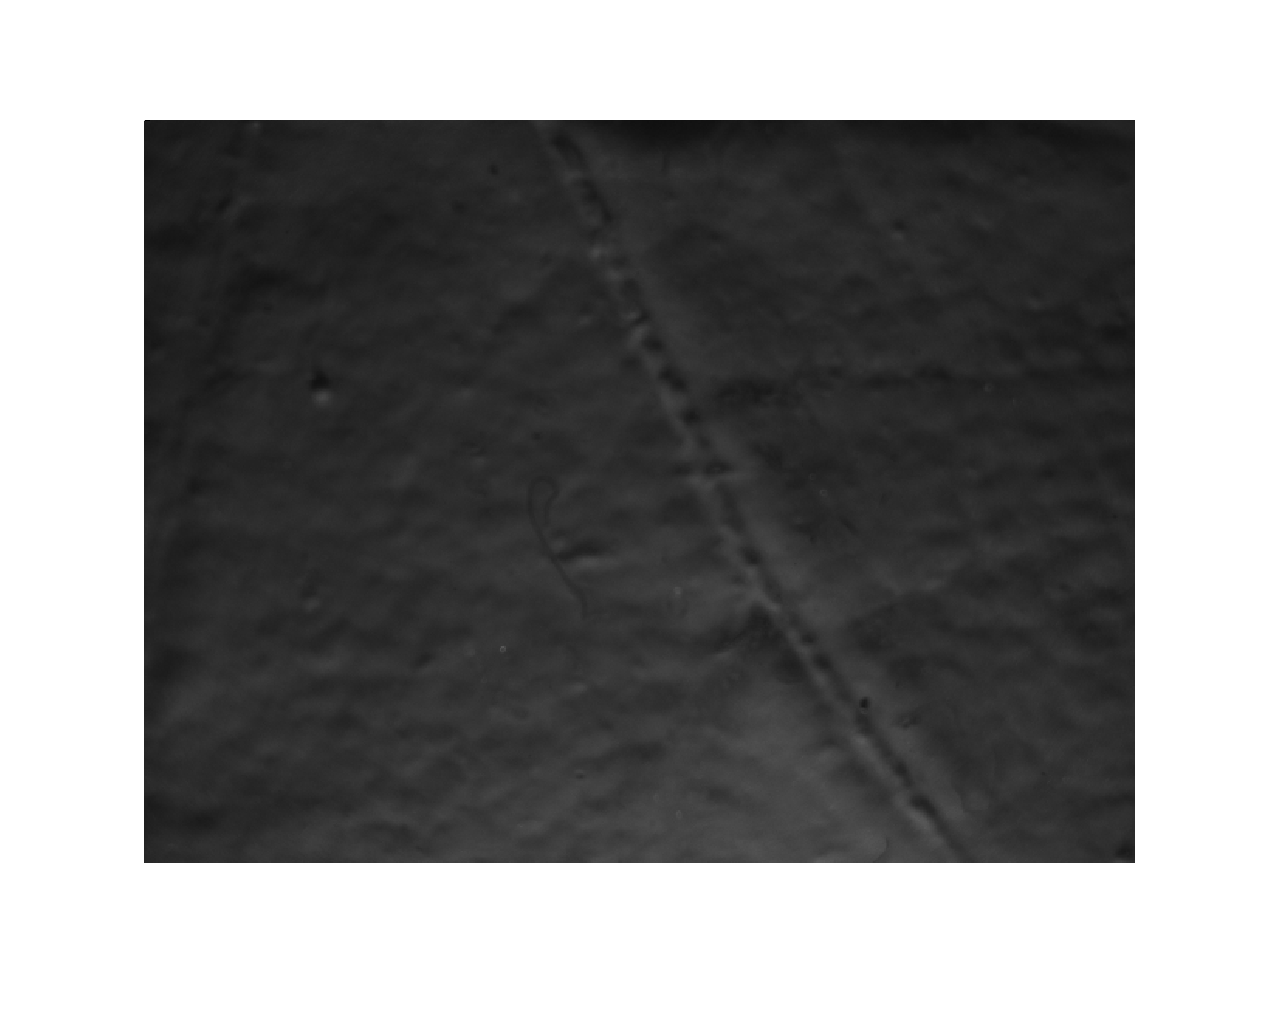
\includegraphics[width=\textwidth]{images/fail_foliage1_lbp.eps}
{\small (e) MH with blur and displaying added "left" RV from multiple boxes}
\endminipage\hfill
\minipage[c]{0.24\textwidth}
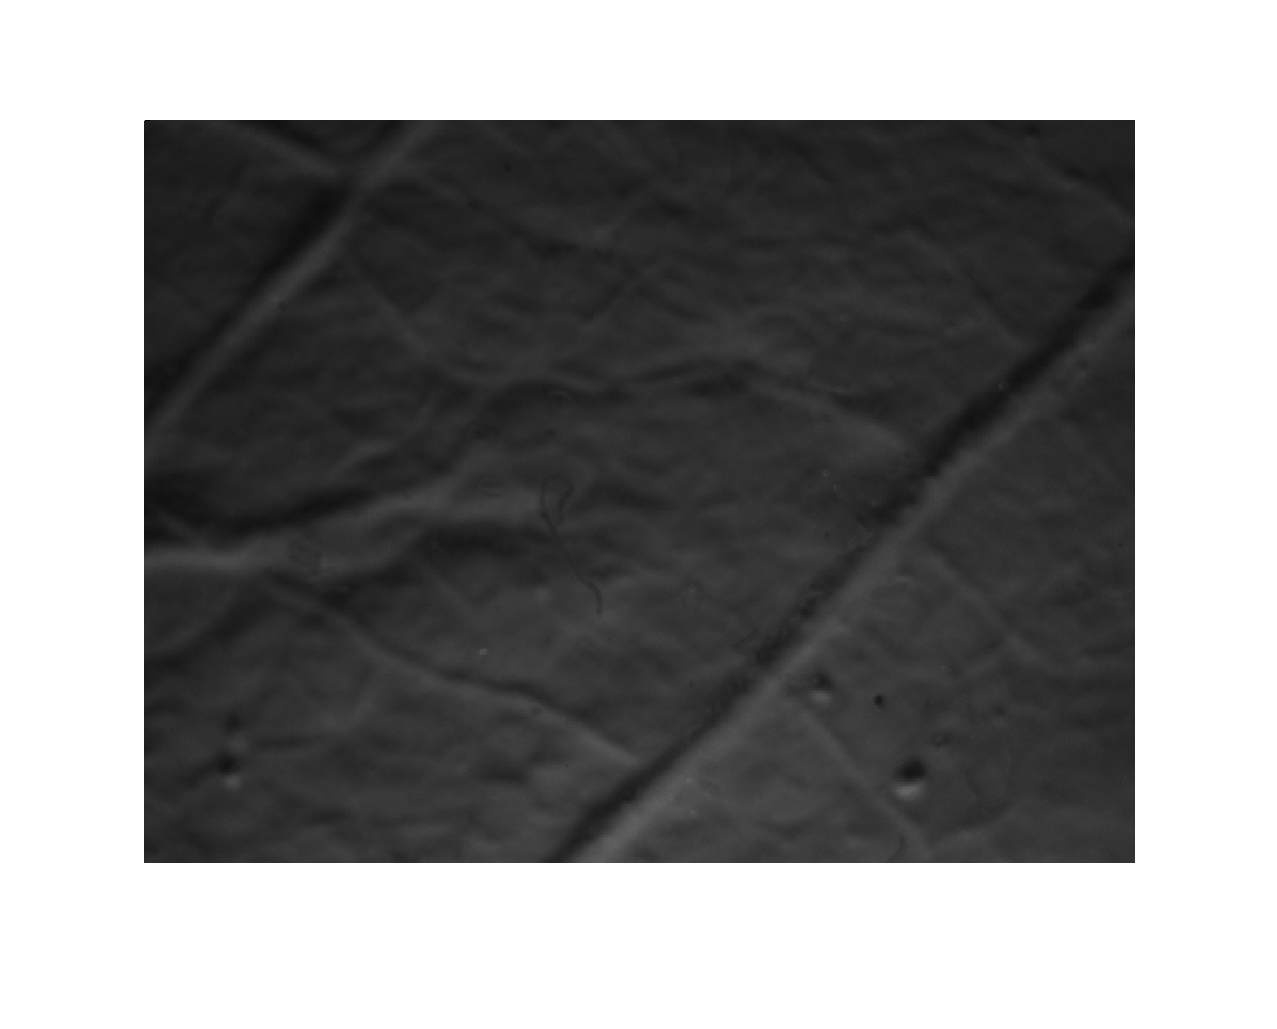
\includegraphics[width=\textwidth]{images/fail_foliage2_lbp.eps}
{\small (f) Gibbs with blur and displaying added "left" RV from multiple boxes}
\endminipage\hfill
\minipage[c]{0.24\textwidth}
\includegraphics[width=\textwidth]{images/fail_foliage1_shape.eps}
{\small (g) MH without blur and displaying added "left" RV from multiple boxes}
\endminipage\hfill
\minipage[c]{0.24\textwidth}
\includegraphics[width=\textwidth]{images/fail_foliage2_shape.eps}
{\small (h) MH sampling without blur and displaying added "left" RV
from multiple boxes}
\endminipage\\

\minipage[c]{0.24\textwidth}
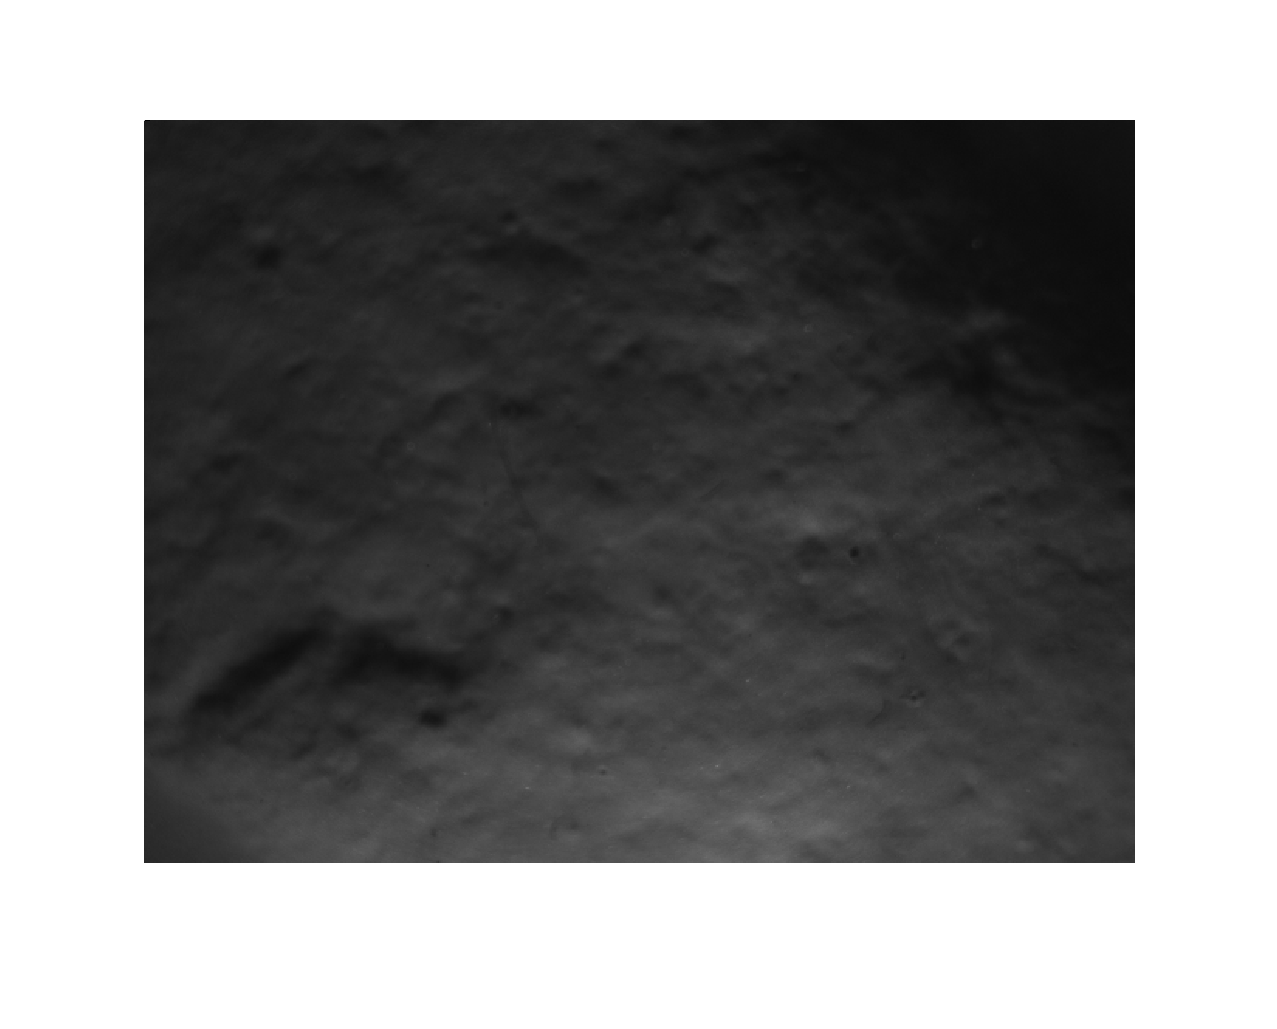
\includegraphics[width=\textwidth]{images/fail_stone1_lbp.eps}
{\small (e) MH with blur and displaying added "left" RV from multiple boxes}
\endminipage\hfill
\minipage[c]{0.24\textwidth}
\includegraphics[width=\textwidth]{images/fail_stone1_shape.eps}
{\small (f) Gibbs with blur and displaying added "left" RV from multiple boxes}
\endminipage\hfill
\minipage[c]{0.24\textwidth}
\includegraphics[width=\textwidth]{images/fail_wood1_shape.eps}
{\small (g) MH without blur and displaying added "left" RV from multiple boxes}
\endminipage\hfill
\minipage[c]{0.24\textwidth}
\includegraphics[width=\textwidth]{images/fail_wood2_shape.eps}
{\small (h) MH sampling without blur and displaying added "left" RV
from multiple boxes}
\endminipage\\

\caption{TODO }
\end{figure*}

%-------------------------------------------------------------------------
\subsection{BLAH}

\begin{table}
\begin{center}
\begin{tabular}{|l|c|}
\hline
Method & Frobnability \\
\hline\hline
Theirs & Frumpy \\
Yours & Frobbly \\
Ours & Makes one's heart Frob\\
\hline
\end{tabular}
\end{center}
\caption{Classification Results.   TODO}
\end{table}


%-------------------------------------------------------------------------
\subsection{Illustrations, graphs, and photographs}

When placing figures in \LaTeX, it's almost always best to use
\verb+\includegraphics+, and to specify the  figure width as a multiple of
the line width as in the example below
{\small\begin{verbatim}
   \usepackage[dvips]{graphicx} ...
   \includegraphics[width=0.8\linewidth]
                   {myfile.eps}
\end{verbatim}
}


%-------------------------------------------------------------------------
\section{Conclusion}

Color is valuable, and will be visible to readers of the electronic copy.
However ensure that, when printed on a monochrome printer, no important
information is lost by the conversion to grayscale.

%------------------------------------------------------------------------
\section{Acknowledgements}

You must include your signed IEEE copyright release form when you submit
your finished paper. We MUST have this form before your paper can be
published in the proceedings.


{\small
\bibliographystyle{ieee}
\bibliography{egbib}
}

\end{document}
